%%
%% Dit is een subdocument van het projectplan.
%%
%%  hier worden tijden en eventueel personen toegekend aan activiteiten
%%


\subsection{Schedule}
 %% dit onderdeel moet vermoedelijk in het schedule plan
  

  \begin{figure}
  	\centering
  	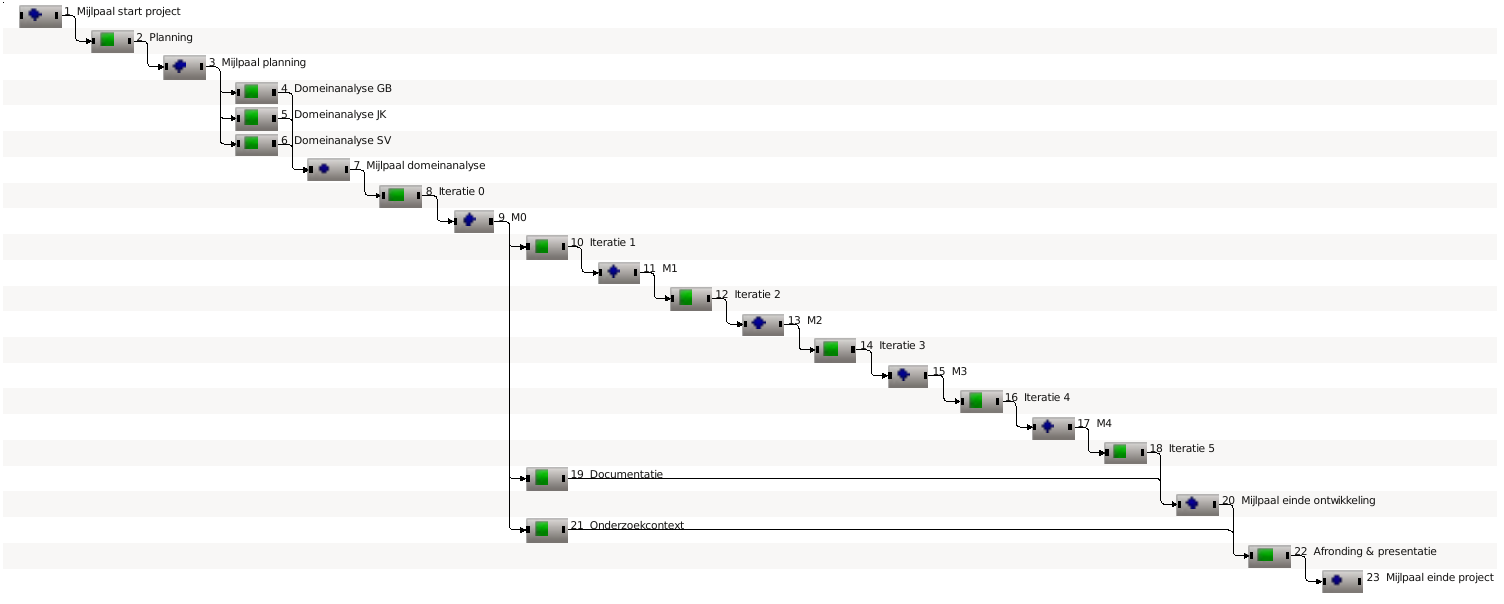
\includegraphics[width=0.8\textwidth,natwidth=1306,natheight=543]{Gantt.png}
  	\caption{\label{fig:Gantt Chart}Scheduling.}
  \end{figure}

\begin{tabular}{ll}\hline
{\bf Fase}    & {\bf weken}\\\hline
Planning             & 2,5 \\

Domeinanalyse        & 3 \\
Architectuur         & 3 \\

Iteratie 1           & 3 \\
Iteratie 2           & 3 \\
Iteratie 3           & 3 \\
Iteratie 4           & 3 \\
Iteratie 5           & 3 \\

Onderzoekcontext     &	2 \\

Afronding	     & 1.5 \\
\hline
Totaal               & 27 \\
\end{tabular}



\begin{itemize}
 \item 27 weken * 15 uur/week = 405 uur
 \item 8 maanden, ongeveer 32 weken beschikbaar, dus 5 weken marge
\end{itemize}



\paragraph{Capaciteitsplanning}

\begin{enumerate}
 \item vakanties?
 \item beschikbaarheid Freek en Bernard?
\end{enumerate}

\paragraph{Planning iteraties}
\begin{enumerate}
 \item 3 weken per interatie
 \item hoeveel tijd voor requirements?
 \item hoeveel tijd voor evaluatie?
\end{enumerate}